%%
%% Automatically generated file from DocOnce source
%% (https://github.com/hplgit/doconce/)
%%

% #define PREAMBLE

% #ifdef PREAMBLE
%-------------------- begin preamble ----------------------

\documentclass[%
oneside,                 % oneside: electronic viewing, twoside: printing
final,                   % draft: marks overfull hboxes, figures with paths
10pt]{article}

\listfiles               %  print all files needed to compile this document

\usepackage{relsize,makeidx,color,setspace,amsmath,amsfonts,amssymb}
\usepackage[table]{xcolor}
\usepackage{bm,ltablex,microtype}

\usepackage[pdftex]{graphicx}

\usepackage[T1]{fontenc}
%\usepackage[latin1]{inputenc}
\usepackage{ucs}
\usepackage[utf8x]{inputenc}

\usepackage{lmodern}         % Latin Modern fonts derived from Computer Modern

% Hyperlinks in PDF:
\definecolor{linkcolor}{rgb}{0,0,0.4}
\usepackage{hyperref}
\hypersetup{
    breaklinks=true,
    colorlinks=true,
    linkcolor=linkcolor,
    urlcolor=linkcolor,
    citecolor=black,
    filecolor=black,
    %filecolor=blue,
    pdfmenubar=true,
    pdftoolbar=true,
    bookmarksdepth=3   % Uncomment (and tweak) for PDF bookmarks with more levels than the TOC
    }
%\hyperbaseurl{}   % hyperlinks are relative to this root

\setcounter{tocdepth}{2}  % levels in table of contents

% Tricks for having figures close to where they are defined:
% 1. define less restrictive rules for where to put figures
\setcounter{topnumber}{2}
\setcounter{bottomnumber}{2}
\setcounter{totalnumber}{4}
\renewcommand{\topfraction}{0.95}
\renewcommand{\bottomfraction}{0.95}
\renewcommand{\textfraction}{0}
\renewcommand{\floatpagefraction}{0.75}
% floatpagefraction must always be less than topfraction!
% 2. ensure all figures are flushed before next section
\usepackage[section]{placeins}
% 3. enable begin{figure}[H] (often leads to ugly pagebreaks)
%\usepackage{float}\restylefloat{figure}

% --- fancyhdr package for fancy headers ---
\usepackage{fancyhdr}
\fancyhf{} % sets both header and footer to nothing
\renewcommand{\headrulewidth}{0pt}
\fancyfoot[LE,RO]{\thepage}
% Ensure copyright on titlepage (article style) and chapter pages (book style)
\fancypagestyle{plain}{
  \fancyhf{}
  \fancyfoot[C]{{\footnotesize \copyright\ 2018-2019, Christian Forssén. Released under CC Attribution-NonCommercial 4.0 license}}
%  \renewcommand{\footrulewidth}{0mm}
  \renewcommand{\headrulewidth}{0mm}
}
% Ensure copyright on titlepages with \thispagestyle{empty}
\fancypagestyle{empty}{
  \fancyhf{}
  \fancyfoot[C]{{\footnotesize \copyright\ 2018-2019, Christian Forssén. Released under CC Attribution-NonCommercial 4.0 license}}
  \renewcommand{\footrulewidth}{0mm}
  \renewcommand{\headrulewidth}{0mm}
}

\pagestyle{fancy}


% prevent orhpans and widows
\clubpenalty = 10000
\widowpenalty = 10000

% --- end of standard preamble for documents ---


\usepackage[swedish]{babel}

\raggedbottom
\makeindex
\usepackage[totoc]{idxlayout}   % for index in the toc
\usepackage[nottoc]{tocbibind}  % for references/bibliography in the toc

%-------------------- end preamble ----------------------

\begin{document}

% matching end for #ifdef PREAMBLE
% #endif

\newcommand{\exercisesection}[1]{\subsection*{#1}}

\input{newcommands_keep}

% ------------------- main content ----------------------



% ----------------- title -------------------------

\thispagestyle{empty}

\begin{center}
{\LARGE\bf
\begin{spacing}{1.25}
Learning from data: Why Bayes is Better
\end{spacing}
}
\end{center}

% ----------------- author(s) -------------------------

\begin{center}
{\bf Christian Forssén}
\end{center}

    \begin{center}
% List of all institutions:
\centerline{{\small Department of Physics, Chalmers University of Technology, Sweden}}
\end{center}
    
% ----------------- end author(s) -------------------------

% --- begin date ---
\begin{center}
Sep 23, 2019
\end{center}
% --- end date ---

\vspace{1cm}


\section{Why Bayes is Better (I)}

% !split
\subsection{Quotes from one pioneering and one renaissance Bayesian authority}
Laplace:

\begin{quote}
\emph{"Probability theory is nothing but common sense reduced to calculation."}
\end{quote}


Sivia

\begin{quote}
\emph{"Bayesian inference probabilities are a measure of our state of knowledge about nature, not a measure of nature itself."}
\end{quote}


% !split
\subsection{Advantages of the Bayesian approach}
% !bpop
\begin{enumerate}
\item Provides an elegantly simple and rational approach for answering, in an optimal way, any scientific question for a given state of information. This contrasts to the recipe or cookbook approach of conventional statistical analysis. The procedure is well-defined:
\begin{itemize}

  \item Clearly state your question and prior information.

  \item Apply the sum and product rules. The starting point is always Bayes’ theorem.

\end{itemize}

\noindent
\item For some problems, a Bayesian analysis may simply lead to a familiar statistic. Even in this situation it often provides a powerful new insight concerning the interpretation of the statistic.

\item Incorporates relevant prior (e.g., known signal model or known theory model expansion) information through Bayes’ theorem. This is one of the great strengths of Bayesian analysis.
\begin{itemize}

  \item For data with a small signal-to-noise ratio, a Bayesian analysis can frequently yield many orders of magnitude improvement in model parameter estimation, through the incorporation of relevant prior information about the signal model.

\end{itemize}

\noindent
\item Provides a way of eliminating nuisance parameters through marginalization. For some problems, the marginalization can be performed analytically, permitting certain calculations to become computationally tractable.

\item Provides a way for incorporating the effects of systematic errors arising from both the measurement operation and theoretical model predictions.

\item Calculates probability of hypothesis directly: $p(H_i|D, I)$.

\item Provides a more powerful way of assessing competing theories at the forefront of science by automatically quantifying Occam’s razor.
\end{enumerate}

\noindent
% !epop

The Bayesian quantitative Occam’s razor can also save a lot of time that might otherwise be spent chasing noise artifacts that masquerade as possible detections of real phenomena.

% !split
\paragraph{Occam's razor.}
Occam’s razor is a principle attributed to the medieval philosopher William of Occam (or Ockham). The principle states that one should not make more assumptions than the minimum needed. It underlies all scientific modeling and theory building. It cautions us to choose from a set of otherwise equivalent models of a given phenomenon the simplest one. In any given model, Occam’s razor helps us to "shave off" those variables that are not really needed to explain the phenomenon. It was previously thought to be only a qualitative principle.

% !split

\begin{figure}[!ht]  % 
  \centerline{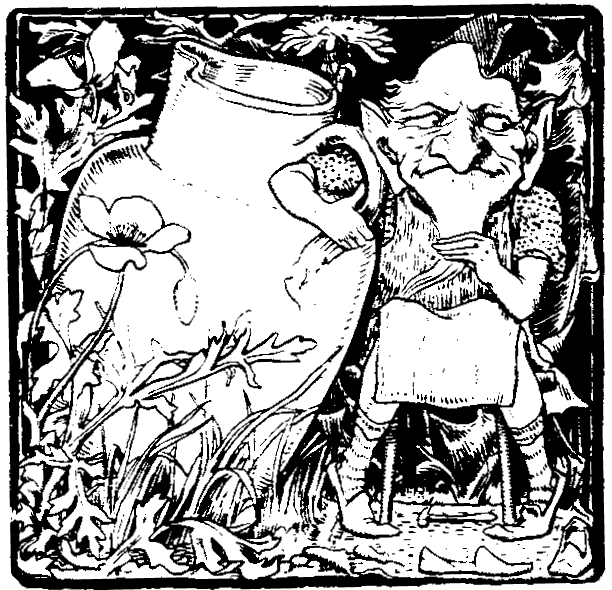
\includegraphics[width=0.7\linewidth]{fig/Leprechaun_or_Clurichaun.png}}
  \caption{
  Did the Leprechaun drink your wine, or is there a simpler explanation?
  }
\end{figure}
%\clearpage % flush figures 


% !split
\subsection{Nuisance parameters (I)}
See demonstration notebook: A Bayesian Billiard game

% !split
\subsection{Nuisance parameters (II): marginal distributions}
Assume that we have a model with two parameters, $\theta0,\theta_1$, although only one of them (say $\theta_1$) is of physical relevance (the other one is a nuisance parameter). Through a Bayesian data analysis we have the joint, posterior pdf
\[
p(\theta_0, \theta_1 | D, I).
\]
The marginal posterior pdf $p(\theta_1 | D, I)$ is obtained via marginalization
\[
p(\theta_1 | D, I) = \int p(\theta_0, \theta_1 | D, I) d\theta_0.
\]
Assume that we have $N$ samples from the joint pdf. This might be the Markov Chain from an MCMC sampler: $\left\{ (\theta_0, \theta_1)_i \right\}_{i=0}^{N-1}$. Then the marginal distribution of $\theta_1$ will be given by the same chain by simply ignoring the $\theta_0$ column, i.e., $\left\{ \theta_{1,i} \right\}_{i=0}^{N-1}$. 

See the interactive demos created by Chi Feng for an illustration of this: \href{{https://chi-feng.github.io/mcmc-demo/}}{The Markov-chain Monte Carlo Interactive Gallery}.

% !split
\subsection{Error propagation (I): marginalization}
The Bayesian approach offers a straight-forward approach for dealing with (known) systematic uncertainties; namely by marginalization. Let us demonstrate this with an example \\

% !split
\textbf{Inferring galactic distances with an imprecise knowledge of the Hubble constant}
The Hubble constant acts as a galactic ruler as it is used to measure astronomical distances according to $v = H_0 x$. An error in this ruler will therefore correspond to a systematic uncertainty in such measurements.

Here we use marginalization to obtain the desired posterior pdf $p(x|D,I)$ from the joint distribution of $p(x,H_0|D,I)$
\[
p(x|D,I) = \int_{-\infty}^\infty dH_0 p(x,H_0|D,I).
\]

Using Bayes' rule: $p(x,H_0|D,I) \propto p(D|x,H_0,I) p(x,H_0|I)$, the product rule: $p(x,H_0|I) = p(H_0|x,I)p(x|I)$, and the fact that $H_0$ is independent of $x$: $p(H_0|x,I) = p(H_0|I)$, we find that
\[
p(x|D,I) \propto p(x|I) \int dH_0 p(H_0|I) p(D|x,H_0,I),
\]
which means that we have expressed the quantity that we want (the posterior of $x$) in terms of quantities that we know.

Assume that the pdf $p(H_0 | I)$ is known via its $N$ samples $\{H_{i}\}_{i=0}^{N-1}$ generated by the MCMC sampler.

This means that we can approximate 
\[
p(x |D,I) \propto \int dH_0 p(H_0|I) p(D|x,H_0,I) \approx \frac{1}{N} \sum_{i=1}^N p(D | x, H_i, I)
\]
where we have used a uniform prior for the distance $p(x|I) \propto 1$.


% !split
\subsection{Error propagation (II): prior information}

\paragraph{Example 3.6.2 in Sivia.}
\begin{itemize}
\item Consider a Bragg peak amplitude that is proportional to the square of a complex structure function: $A = f^2$.

\item The amplitude is measured with an uncertainty $A = A_0 \pm \sigma_A$ from a least-squares fit to experimental data.

\item What is $f = f_0 \pm \sigma_f$?
\end{itemize}

\noindent
See notes and demonstration notebook.

% ------------------- end of main content ---------------

% #ifdef PREAMBLE
\end{document}
% #endif

